\documentclass{amsart}
%\documentclass[smallextended,nospthms]{svjour3}
\usepackage{mathptmx,tikz}
\pgfrealjobname{figure}
\begin{document}
% -- pdflatex --jobname=figure1 figure.tex
\beginpgfgraphicnamed{figure1}
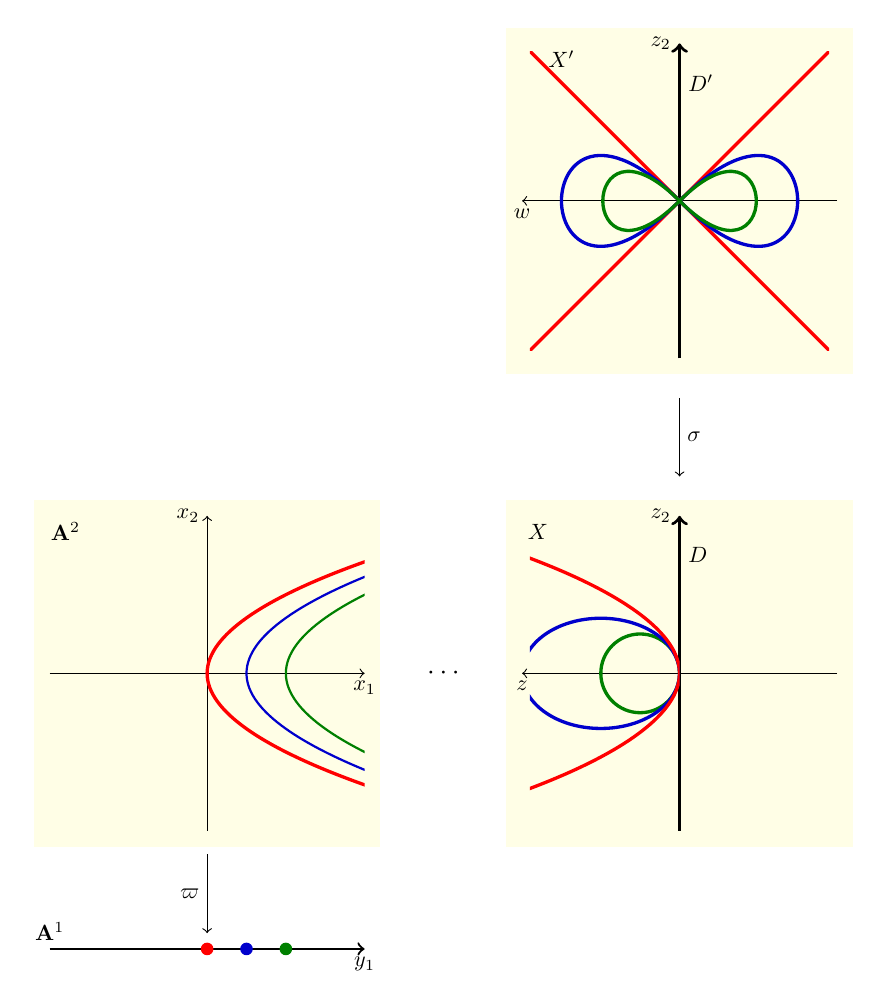
\begin{tikzpicture}
% left picture
\begin{scope}[xshift=-3cm,yshift=-3cm]
\fill[color=yellow!10] (-2.2,-2.2) rectangle (2.2,2.2);

\draw[->] (-2,0) -- (2,0) node [below,at end,scale=0.8] {$x_1$};
\draw[->] (0,-2) -- (0,2) node [left,at end,scale=0.8] {$x_2$};
\draw (-1.8,1.8) node [scale=0.8] {$\mathbf{A}^2$};
% we draw three parabolas. Note that the tikz command "parabola" draws y=x^2, hence we have to rotate the picture by -90 degrees.
% we can add more parabolas
\begin{scope}
\clip (-2,-2) rectangle (2,2);
\draw[color=red,very thick,rotate=-90] (-2,4) parabola bend (0,0) (2,4);
\draw[color=blue!80!black,thick,rotate=-90] (-2,4.5) parabola bend (0,0.5) (2,4.5);
\draw[color=green!50!black,thick,rotate=-90] (-2,5) parabola bend (0,1) (2,5);
\end{scope}
\begin{scope}[yshift=-0.5cm] % the first attempt was close to the picture, we move the A1 line slightly down
\draw[thick,->](-2,-3) -- (2,-3) node [at end, below,scale=0.8]{$y_1$} node [above, at start, scale=0.8]{$\mathbf{A}^1$};
\fill[draw=none,color=red](0,-3) circle (0.08cm);
\fill[draw=none,color=blue!80!black](0.5,-3) circle (0.08cm);
\fill[draw=none,color=green!50!black](1,-3) circle (0.08cm);
\end{scope}
\draw[->] (0,-2.3) -- (0,-3.3) node [midway,scale=0.8,left] {$\varpi$};
\end{scope}

\draw (0,-3) node {$\cdots$};

% bottom right picture
\begin{scope}[xshift=3cm,yshift=-3cm]
\fill[color=yellow!10] (-2.2,-2.2) rectangle (2.2,2.2);
\draw[->] (2,0) -- (-2,0) node [below,at end,scale=0.8] {$z$};
\draw[very thick,->] (0,-2) -- (0,2) node [left,at end,scale=0.8] {$z_2$} node [right, very near end, scale=0.8] {$D$};
\draw (-1.8,1.8) node [scale=0.8] {$X$};
%we will draw circles. This is easy, but we have to clip the part of the picture
\begin{scope}
\clip (-1.9,-2) rectangle (0,2);
\draw[very thick,green!50!black] (0,0) arc [start angle=0,end angle=360, radius=0.5cm]; %tikz draws arcs from the starting point.
%\draw[very thick,blue!80!black] (0,0) arc [start angle=0,end angle=360, radius=0.8cm];
\draw[very thick,blue!80!black] (-1,0) ellipse (1cm and 0.7cm);
\draw[color=red,very thick,rotate=90] (-1.5,2) parabola bend (0,0) (1.5,2);
%\draw[very thick,green!50!black] (0,0) arc [start angle=0,end angle=360, radius=1.5cm];
\end{scope}
\end{scope}

% top right
\begin{scope}[xshift=3cm, yshift=3cm]
\fill[color=yellow!10] (-2.2,-2.2) rectangle (2.2,2.2);
\draw[->] (2,0) -- (-2,0) node [below,at end,scale=0.8] {$w$};
\draw[very thick,->] (0,-2) -- (0,2) node [left,at end,scale=0.8] {$z_2$}node [right, very near end, scale=0.8] {$D'$};;
\draw (-1.5,1.8) node [scale=0.8] {$X'$};
% we clip again the bezier curves
\begin{scope}
\clip (-1.9,-1.9) rectangle (1.9,1.9);
\draw[very thick, red] (-2,2) -- (2,-2);
\draw[very thick, red] (-2,-2) -- (2,2);
%
\draw[very thick, blue!80!black] (0,0) .. controls (2,2) and (2,-2) .. (0,0);
\draw[very thick, blue!80!black] (0,0) .. controls (-2,2) and (-2,-2) .. (0,0);
%
\draw[very thick, green!50!black] (0,0) .. controls (1.3,1.3) and (1.3,-1.3) .. (0,0);
\draw[very thick, green!50!black] (0,0) .. controls (-1.3,1.3) and (-1.3,-1.3) .. (0,0);
\end{scope}
\end{scope}

\draw[->] (3,0.5) -- (3,-0.5) node [right,midway,scale=0.8] {$\sigma$};
%\clip(-2,-2) rectangle (6,2);
%\fill[color=yellow!10](-2,-1.5) rectangle (6,1.5);
%\begin{scope}
%\clip (0,-1.5) rectangle (5,1.5);
%\fill[color=orange!30] (0,0) .. controls (2,0) and (5,1) ..  (6,1) -- (6,-2) -- (0,-2) -- (0,0);
%\fill[color=yellow!10] (0,0) .. controls (2,0) and (5,-1) .. (6,-1) -- (6,-2) -- (0,-2) -- (0,0);
%\end{scope}
%\draw[blue,thick] (0,0) .. controls (2,0) and (5,1) .. node[below,at end,scale=0.8]{$z_+$} (6,1);
%\draw[violet,thick] (0,0) .. controls (2,0) and (5,-1) .. node[below,at end,scale=0.8]{$z_-$}  (6,-1);
%
%
%\draw[red, thin] (-1,1.5) .. controls (-0.5,1) and (0,0) .. (1,0) .. controls (1.5,0) and (1.5,1) .. (2,1) .. controls (3,1) and (5,0.5) .. (6,0.5);
%\draw[red,thin] (-2,1) .. controls (-1,1) and (1.5,0.5).. (2,0.5) ..controls (3,0.5) and (5,-0.5) .. (6,2);
%\draw[green!70!black,thin] (-2,-1) .. controls (-1.5,-1) and (0.5,0) .. (1,-0.3) .. controls (1.5,-0.6) and (4,0.3) .. (6,-1.5) ;
%\draw[green!70!black,thin] (-2,0.5) .. controls (-1,-0.5) and (1,0) .. (1.5,0) .. controls (2,0) and (3,-1) .. (3.5,-1) .. controls (4,-1) and (5,0) .. (6,0);
%%\draw[red,thick] (-1,-1) .. controls (-0.5,-0.5) and (-0.5,0.5) .. node[near end,left,scale=0.8]{$z_i$} (0,1);

\end{tikzpicture}
\endpgfgraphicnamed
\end{document}
